\section{System Overview}
In this section we provide an user level description of our system. In the next section we deep down into the system architecture and explain why it perform high.
\subsection{Process Graph}
A Process graph (Figure \ref{processgraph}) mainly consists of the Adapters and the processors which does the processing logic for the system. Adapters are used to receive events from out side sources. Processors will receive events from other processors and output events to be consumed by other processors. 

\begin{figure}
        \centering
        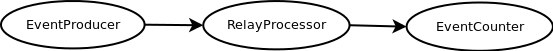
\includegraphics[width=0.6\textwidth]{processgraph.png}
        \caption{Process Graph}
        \label{processgraph}
\end{figure}

\subsection{}